The large mean free path $\lambda$ allows the electrons - on the contrary to the ions - to gain
significant energy in the electric field. They can reach up to several keV so that their
deBroglie-wavelength is in the range of the atom's diameter. Quantum mechanical effects
of interference lead to strong dependencies of the collision cross section $\sigma$ of the kinetic
energies of the electrons and therefore to the mean free path $\lambda\approx
1/\sigma$.

\begin{figure}[htbp]
	\begin{minipage}[b]{0.65\textwidth}
		\begin{figure}[H]
		\centering
		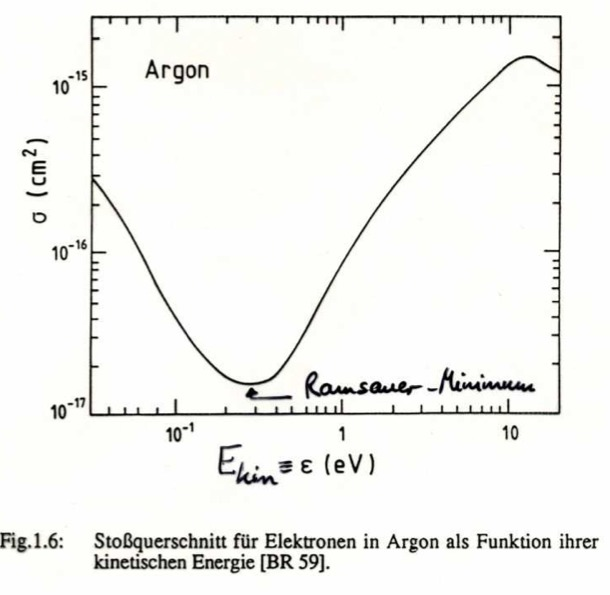
\includegraphics[width=\textwidth]{Fig-03-06.jpg}
		\end{figure}
	\end{minipage}
	\hspace{0.5cm}
	\begin{minipage}[b]{0.25\textwidth}
		\begin{figure}[H]
		\centering
		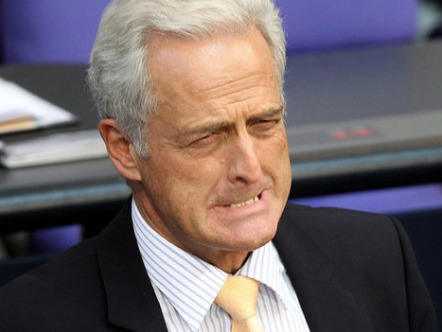
\includegraphics[width=\textwidth]{Fig-03-10a.jpg}
		\end{figure}
	\end{minipage}
	\caption{b}
	\label{rekristall} 
\end{figure}

To derive a estimation of the drift velocity of the electrons under influence of an electric field,
we consider a group of electrons with thermal velocity of 

\[u=\sqrt{\frac{2E_{\text{kin}}}{m}}  \]

which move away istotropically from a point $P$:

\begin{figure}[H]
	\centering
	
\includegraphics[width=0.5\textwidth]{dummy.jpg}
\end{figure}

In an electric field $\vec{E}$, the radial pathways become parabolic pathways (acceleration
$\vec{b}=q\vec{E}/m$).

\begin{figure}[H]
	\centering
	
\includegraphics[width=0.5\textwidth]{dummy.jpg}
\end{figure}

$\delta_z$ is the shifting of $D+D_E$ along the z-axis.
\\
The averaging over all cos$\,\Theta$ yields

\[ \langle \delta_z \rangle = \frac{1}{3}\cdot \frac{qE}{m}\cdot \langle t^2 \rangle \]

For $\langle t^2 \rangle$, we obtain with averaging over all durations for all free paths $s$ and
the thermal electron velocity $u$:

\[ \langle t^2 \rangle = \frac{\langle s^2 \rangle}{u^2} = \frac{2\lambda_e^2}{u^2} ,\]

while we assumed that  $\lambda_e$ is independant of $u$ (i.e. the collision cross section $\sigma$
is independent of $u$). With that, we obtain for the drift velocity ($\langle t
\rangle=\lambda_e/u$):

\[v_D = \frac{\langle \delta_z \rangle}{\langle t\rangle} = \frac{2}{3}\cdot \frac{qE}{m}\cdot
\frac{\lambda_e}{u}\]

It should be noted that $\lambda\sim \frac{1}{\text{pressure }p}$, so that $v_D$ is explicitly
dependant of the reduced field strength $E/p$.
\\
A constant drift velocity requires equality of the gain of energy in the field $E-$ and the loss of
energy through collisions:

\[qE\cdot v_D\cdot \tau = \Delta(E_\text{kin})\cdot E_\text{kin}  \]

with $\tau$ as time between two collisions and the fraction of the energy $\Delta(E_\text{kin})$
that is transferred to the gas atom during the collision. We obtain

\[qE\cdot v_D = \frac{\Delta(E_\text{kin})\cdot E_\text{kin}}{\tau} =
\frac{\Delta(E_\text{kin})\cdot E_\text{kin}\cdot u}{\lambda_e}  ,\]

which continues to 

\[qE\cdot v_D = \left\langle \frac{\Delta(E_\text{kin})\cdot E_\text{kin}}{\tau} \right\rangle =
\left\langle \frac{\Delta(E_\text{kin})\cdot E_\text{kin}\cdot u}{\lambda_e}\right\rangle .\]


